\begin{sectionbox}
    \subsection{Feldverhalten an Materialgrenzen}
    \begin{center}
        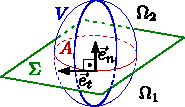
\includegraphics{./img/boundary.pdf}
    \end{center}
    Sprungbedingung für die Normalenableitung des Potentials:\\
    \begin{eqnarray*}
        \epsilon_1\frac{\partial \Phi}{\partial n}\big|_1 - \epsilon_2\frac{\partial \Phi}{\partial n}\big|_2 = \sigma_{\ir int} \text{ auf }\Sigma\\
    \end{eqnarray*}
    An Grenzflächen gibt es Flächenladung $\sigma:$ \\
    $Q = \lim\limits_{h \ra 0} \int_V \rho \diff V = \int_A \sigma \diff \vec a$\\

    Die Tangentialkomponente des E-Feldes\\ und die Normalkomponente des B-Feldes sind stetig
    \begin{eqnarray*}
        \vec D_2 \vec n - \vec D_1 \vec n = \sigma_{\ir int} \\
        \vec B_2 \vec n - \vec B_1 \vec n = 0 \\
        \vec E_1 \times \vec n - \vec E_2 \times \vec n = 0 \\
        \vec H_2 \times \vec n - \vec H_1 \times \vec n = \vec j
    \end{eqnarray*}
    Brechungsgesetz für elektrische Feldlinien (2 Isolatoren): \\
    \begin{eqnarray*}
        \frac{\tan \alpha_1}{\tan \alpha_2} = \frac{\varepsilon_1}{\varepsilon_2}
    \end{eqnarray*}
    Gleiches gilt für $\vec j = 0$ auch für das $\vec B$ bzw. $\vec H$-Feld
\end{sectionbox}